\begin{figure}
  \centering
  \subfloat[Distribuição de todas as amostras de áudio]{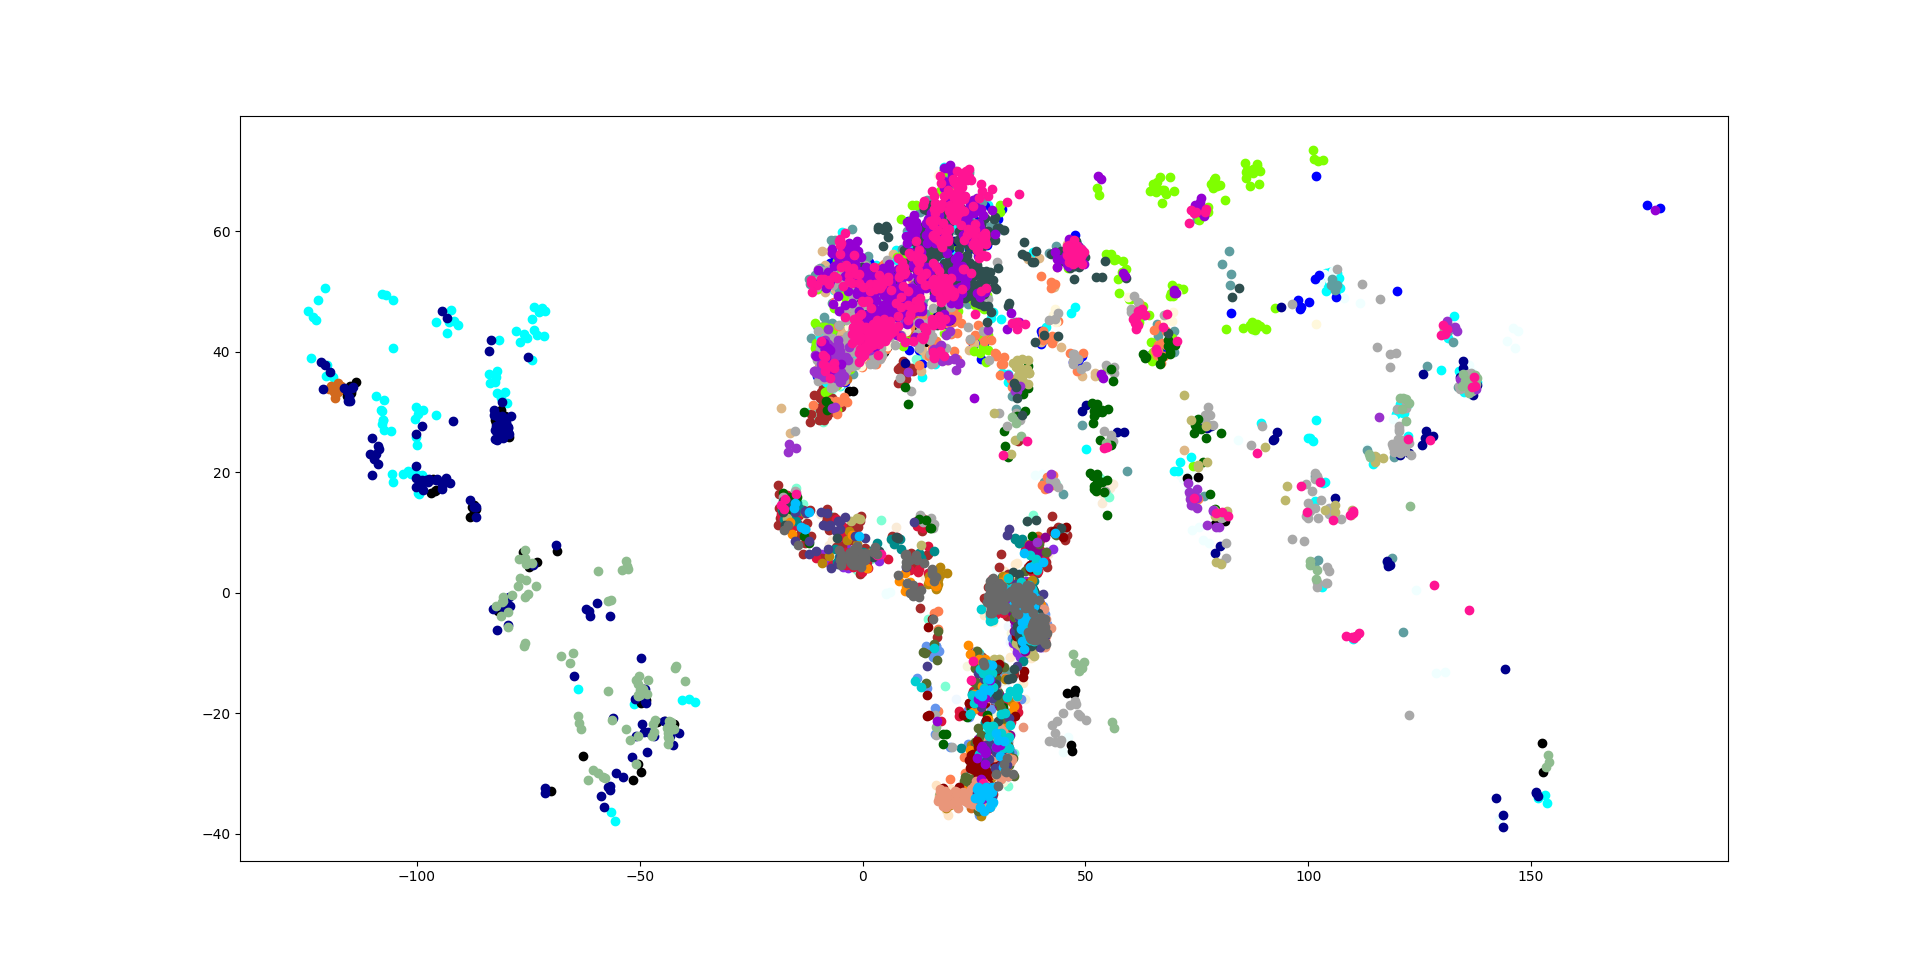
\includegraphics[width=0.8\columnwidth]{figuras/geral.png}}
  \hfill
  \subfloat[Distribuição dos pontos de referência de cada classe]{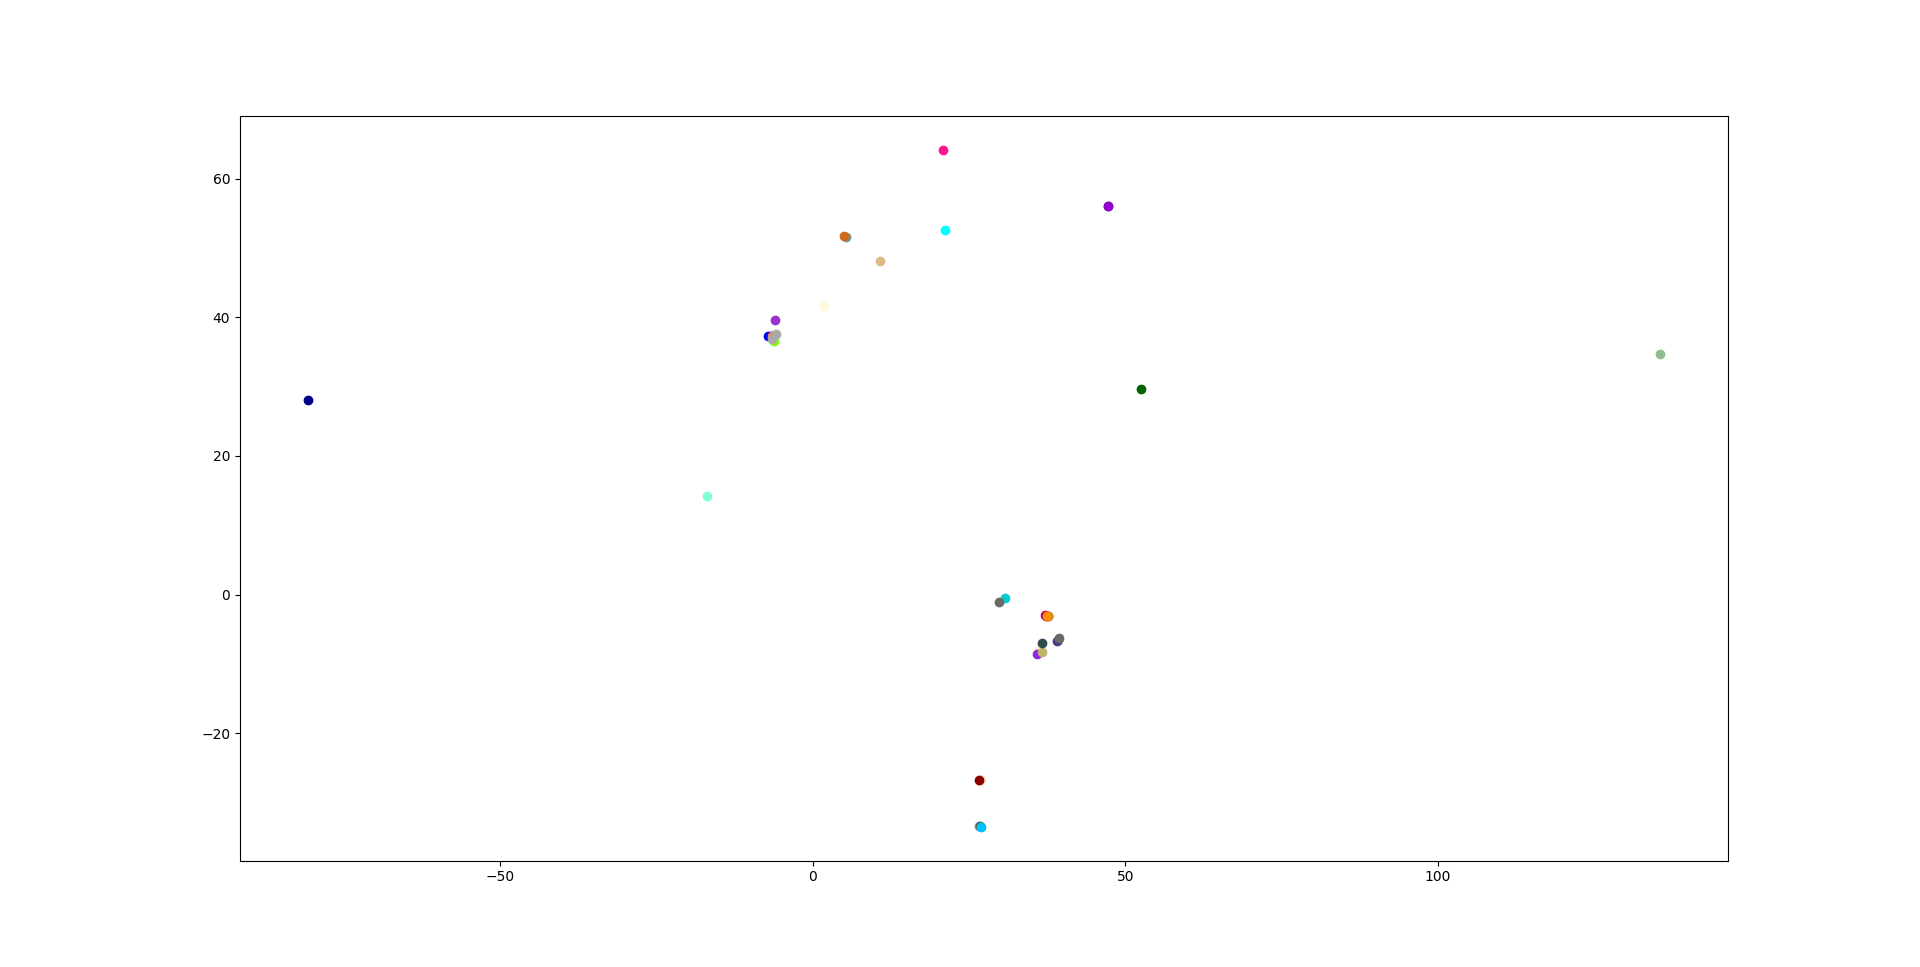
\includegraphics[width=0.8\columnwidth]{figuras/pontos.png}}
  \hfill
  \subfloat[Ponto de referência a ser analisado]{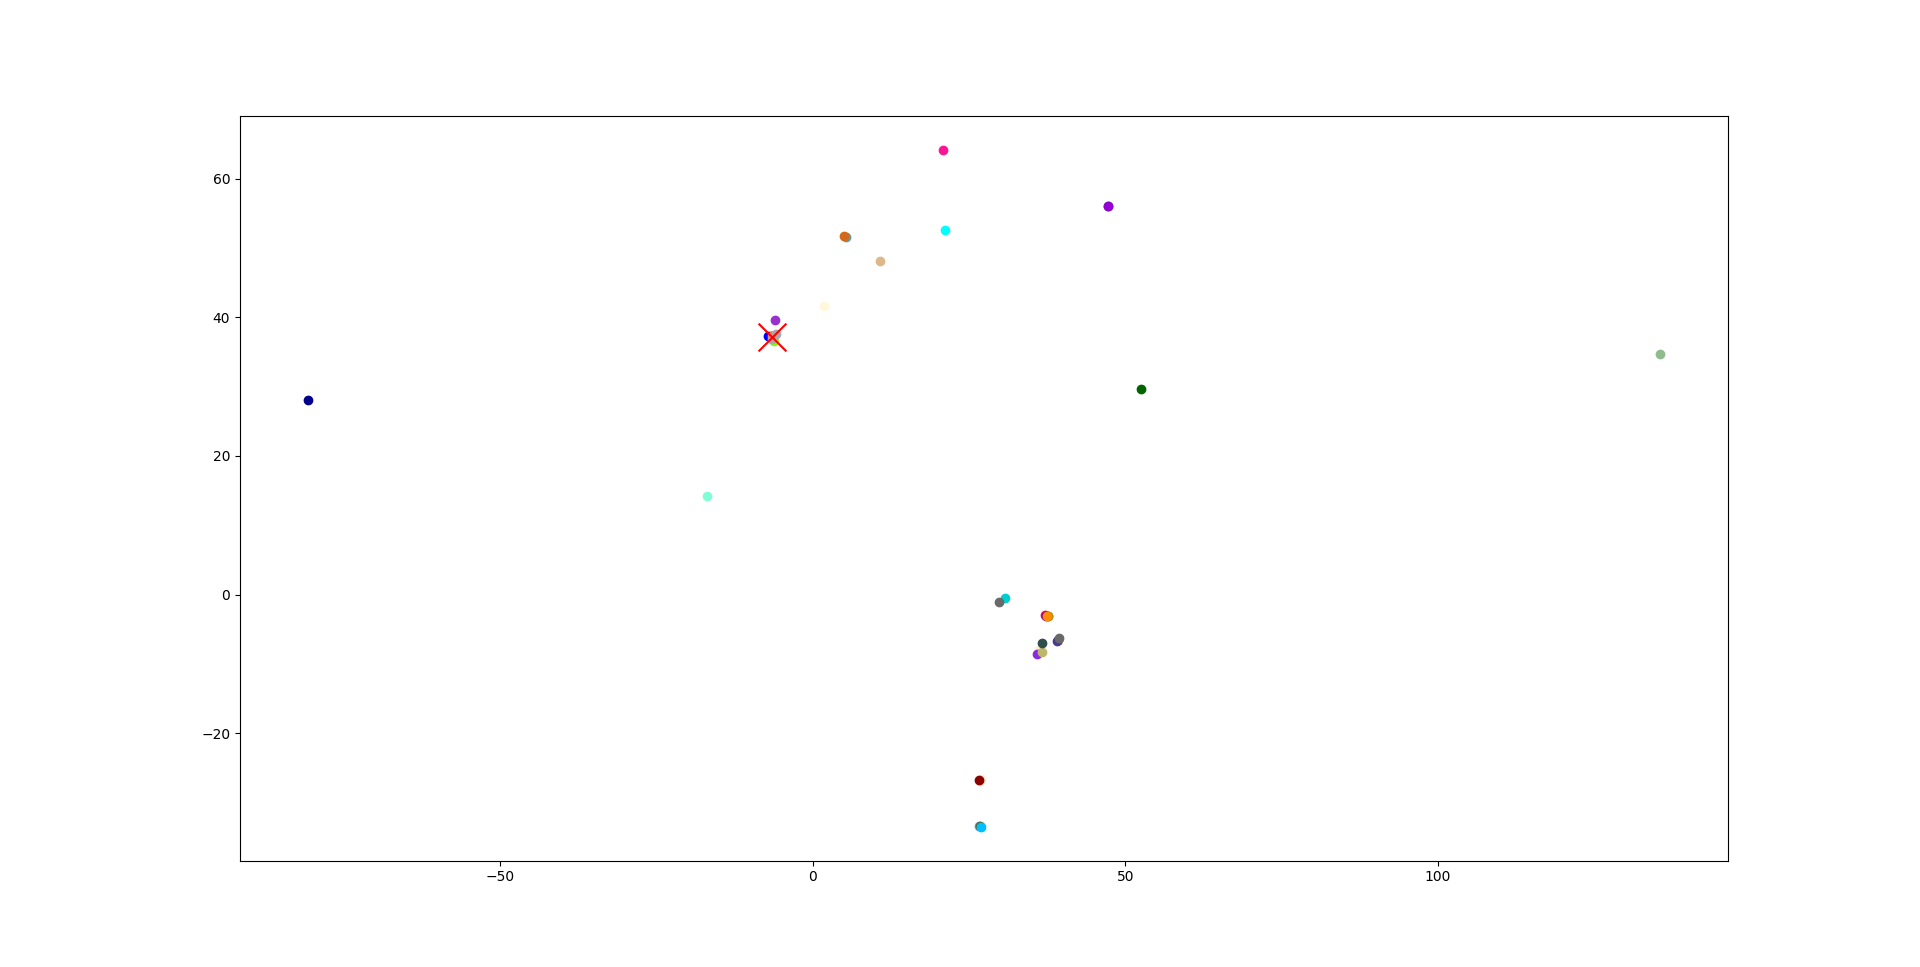
\includegraphics[width=0.8\columnwidth]{figuras/referencia.png}}
  \hfill
  \caption{Mapeamento das amostras de áudio}
  \label{fig:three graphs}
\end{figure}